\newpage
\subsubsection{Creating EReferences with MOSL}
\texHeader
\hypertarget{static:references tex}{}

% Add quote environment
In MOSL, the declaration of a reference is simple - you simply set each of the properties we discussed in the following syntax: {\small{\texttt{[Aggregation
Type][Navigation Name](Multiplicity):[Source role]}}}. The source type is determined by the class in which the reference is placed. Aggregation
is defined a sideways diamond.

\begin{itemize}

\item[$\blacktriangleright$] Open \texttt{Box.eclass} in the editor and add a \emph{container reference} named \texttt{containedPartition} with a
multiplicity of zero to infinity, from \texttt{Box} to \texttt{Partition} (Fig.~\ref{fig:cpartitionReference}). This means a \texttt{Box} can hold an
infinite number of partitions.

\begin{figure}[htbp]
	\centering
  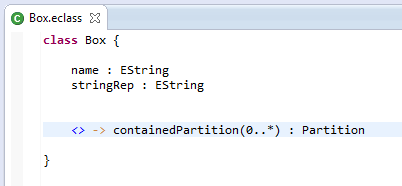
\includegraphics[width=0.6\textwidth]{eclass_box}
	\caption{Creating a \emph{contained reference} in \texttt{Box}}
	\label{fig:cpartitionReference}
\end{figure} 

\item[$\blacktriangleright$] Now add a \emph{simple reference} to \texttt{Partition}. Name it \texttt{box}, and allow it to hold up to one \texttt{Box}
(Fig.~\ref{fig:boxReference}). This means a single partition can belong to either zero, or one \texttt{Box}, and that's it. It can't belong to two different
boxes at the same time.

\begin{figure}[htbp]
	\centering
  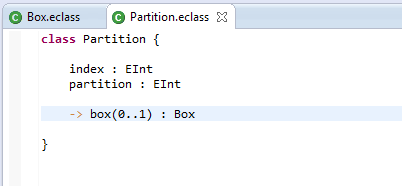
\includegraphics[width=0.6\textwidth]{eclass_partition}
	\caption{Creating a \emph{simple reference} in \texttt{Partition}}
	\label{fig:boxReference}
\end{figure} 

\item[$\blacktriangleright$] Congratulations, you have just built your first pair of EReferences! To see how this is depicted visually, check out
Fig.~\ref{fig:ereference_completed} from the previous subsection.

\newpage

\item[$\blacktriangleright$] Now, lets create another pair of EReferences between \texttt{Partition} and \texttt{Card}. If you think about it, it's really not
all that different from the relation between \texttt{Box} and \texttt{Partition}. A \texttt{Partition} should be able to hold an unlimited amount of
\texttt{Card}s, but a \texttt{Card} should only be allowed to belong to zero or one \texttt{Partition}s. Name the two new references
\texttt{containedPartition}, and \texttt{box}. Your classes should now closely resemble Fig.~\ref{fig:almostAllReferences}.

\begin{figure}[htbp]
	\centering
  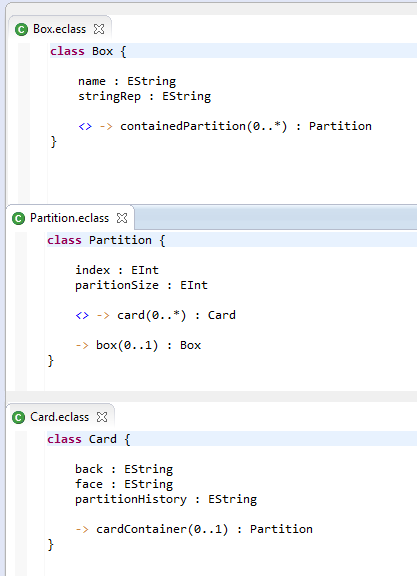
\includegraphics[width=0.65\textwidth]{eclipse_workspaceReferences}
	\caption{The Completed Bidirectional EReferences}
	\label{fig:almostAllReferences}
\end{figure} 

\item[$\blacktriangleright$] The next step is to set up two connections between \texttt{Partition}s and, so \texttt{Cards} can be moved between its previous and
next partitions in the box. Create two new simple references, named \texttt{previous}, and \texttt{next}, each with a \texttt{0..1} multiplicity. Allow them to
have a maximum of 1 link each.

\item[$\blacktriangleright$] If you have done everything correctly, your classes should now resemble Fig.~\ref{fig:allReferences}. 

\begin{figure}[htbp]
	\centering
  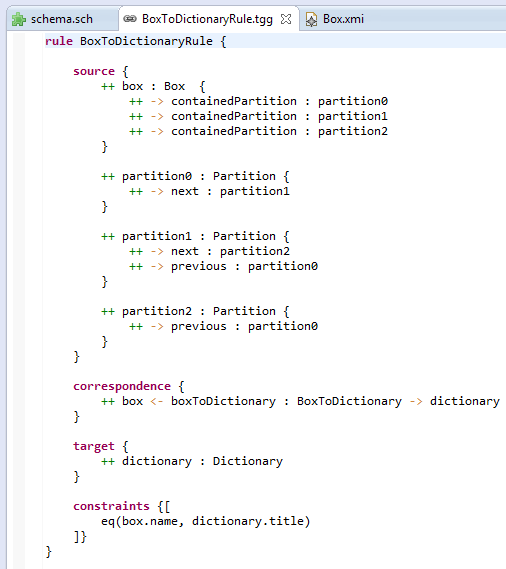
\includegraphics[width=0.6\textwidth]{eclipse_allReferences}
	\caption{All references for our Leitner's Learning Box}
	\label{fig:allReferences}
\end{figure} 

\newpage

At this point, all of your references have been created! The problem is, suppose you set the \texttt{containedPartition} reference in a particular \texttt{Box}.
That's great, you would now have the box containing one partition. However, if you went and examined that partition independently, its \texttt{box} reference
would still be null. We still need to set up the link between these references so that when one is updated, the other will be too.

\item[$\blacktriangleright$] Navigate to the ``\_constraints.mconf'' file. You can see it has a single \texttt{opposites} scope that's currently empty. Enter
the following text: \texttt{containedPartition : Box <-> box : Partition}. This statement sets the two references to be opposites of one another, i.e., the
connection between the classes is now bidirectional.

\item[$\blacktriangleright$] Reviewing the \texttt{Partition} class, its easy to see that \texttt{previous} and \texttt{next} are certainly not opposites
(Fig.~\ref{}), but we do need to establish the same opposite link between a \texttt{card} and its \texttt{cardContainer}. Follow the same steps until your
constraint file resembles Fig.~\ref{fig:bothConstraints}.

\begin{figure}[htbp]
	\centering
  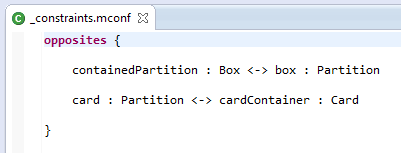
\includegraphics[width=0.6\textwidth]{eclipse_workspaceBothConstraints}
	\caption{The completed constraints file}
	\label{fig:bothConstraints}
\end{figure} 

\item[$\blacktriangleright$] Now the references for your Leitners learning box are truly complete! To see how each of the classes, attributes, and references
are depicted in the visual syntax, check out Fig.~\ref{fig:ereferences_all} in \hyperlink{sec:static vis}{Section 2.1}. Otherwise, build your project to
make sure there are no errors, and continue to the next section to finalize the declaration of your classes.

\fancyfoot[R]{$\triangleright$ \hyperlink{static:methods tex}{Next}}

\end{itemize}
